\documentclass{article}
\usepackage{geometry}
\usepackage{graphicx}
\geometry{
	a4paper,
	total={170mm,257mm},
	left=30mm,
	top=30mm,
	bottom=20mm,
	right=20mm
}
\title{Álgebra Aplicada à Música}
\date{2022-07-13}
\author{Paulo Roberto Rodrigues da Silva Filho - DRE: 122065831}

\begin{document}
	\renewcommand{\figurename}{Figura}
	\graphicspath{ {./imagens/} }
	\maketitle
	\tableofcontents
	\section{Introdução}
	
	\paragraph{}
	Foi apresentado nesse seminário o trabalho do Prof. Dr. Carlos Mathias, docente da Universidade Federal Fluminense.
	
	\paragraph{}
	O Prof. Carlos Mathias é Graduado, Mestrado e Doutorado na UFRJ e tem trabalhado ao longo de sua carreira envolvido com educação e com iniciativas do que é chamado de Matemática Humanista, que considera não apenas aspectos educacionais e metodológicos do ensino da matemática, mas também aspectos corporais e emocionais.
	
	\paragraph{}
	O projeto DRUMMATH, de ensino de música para deficientes visuais, aplica a aritmetização da música para esses objetivos, também foi apresentado nesse seminário.
	
	\section{Aritmética da Música}
	
	\paragraph{}
	O seminário foi iniciado com a apresentação do modelo de aritmetização da música. Essa aritmetização é feita através da definição de um valor inteiro que representa o período inteiro de tempo, para um ciclo rítmico. É definido ritmo a repetição de sons periodicamente.
	
	\begin{figure}[h]
		\centering
		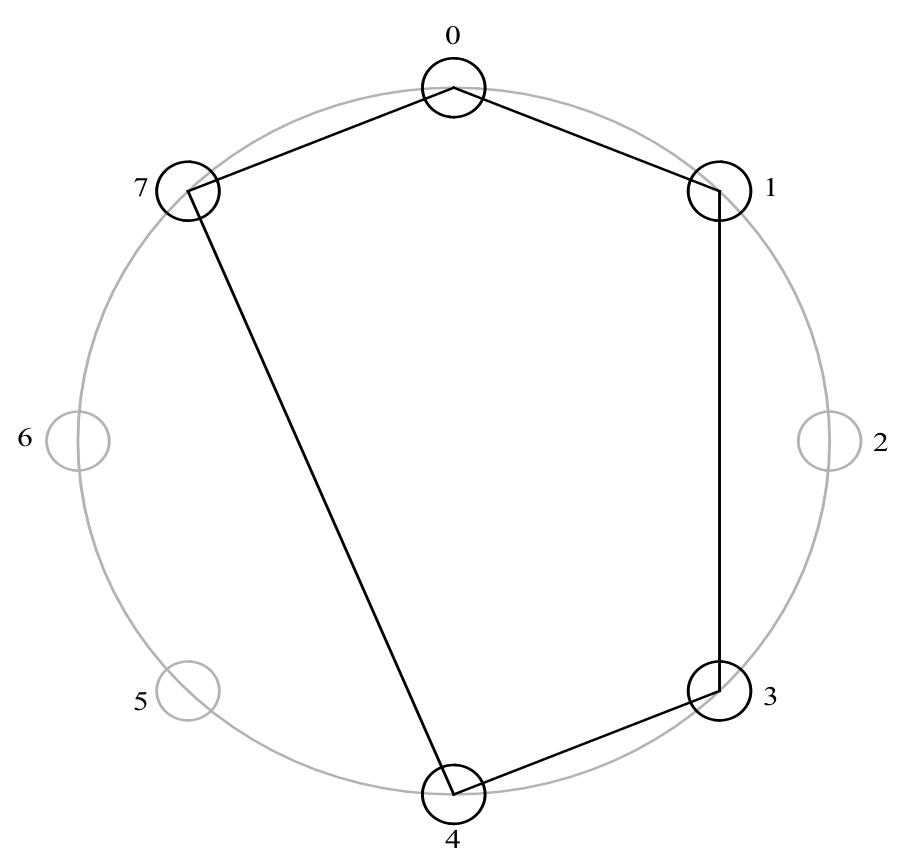
\includegraphics[scale=0.7]{7-Cycles}
		\caption{Exemplo de música com tempo igual a 7, e marcações nas posições 0, 1, 3, 4 e 7, que correspondem a sequencia dos números inteiros \textit{X \textbf{mod} 7}}
		\label{Figura-1}
	\end{figure}
	
	\paragraph{}
	Um período inteiro é representado por um número. Na Figura \ref{Figura-1} acima, um período é representado pelo número \textit{7}, com batidas em todos os tempos \textit{0, 1, 3, 4 e 5 \textbf{mod} 7}.
	
	\paragraph{}
	A aritmetização dos ritmos permitem a comparação, \textit{encoding}, produção, arranjo de músicas. Além disso, uma vez entendidos os ritmos, é possível fazer o processo inverso: a partir das músicas, entender os princípios de congruência e divisibilidade. É aí que entra o projeto DRUMMATH.
	
	\section{O Projeto DRUMMATH}
	
	\paragraph{}
	O Projeto DRUMMATH, aplicado no Instuto Benjamin Constant, para Deficientes Visuais, no Rio de Janeiro, utiliza-se da música e de aspectos sensoriais para o ensino de Matemática básica a deficientes visuais.
	
	\paragraph{}
	Como foi apresentado na seção anterior, os ritmos podem ser aritmetizados, e, dado um período de tempo, é possível mostrar os conceitos de divisão, contagem, multiplicação e divisão, sem a necessidade de aparatos visuais, utilizando-se apenas aparatos auditivos.
	
	\paragraph{}
	Com a variação da frequência dos sons, relacionados à extensão da onda, e dos equipamentos que geram tais sons, é possível identificar extensão de objetos grandes (como mesas, por exemplo), além de utilizarmos diferentes combinações rítmicas para representar somas, subtrações e divisões, utilizando a música para representar conceitos de aritmética.
	
	\paragraph{}
	Assim, o projeto DRUMMATH parte da música para a aritmética, sendo uma aplicação inversa da aritmetização rítmica, mas com fins didáticos e lúdicos.
	
	\section{Outras Aplicações da Aritmetização da Música}
	
	\paragraph{}
	Foi apresentado pelo Prof. Carlos Mathias outras aplicações da aritmetização da música, principalmente para a produção e arranjo musical e para a comparação rítmica.
	
	\paragraph{}
	Foi apresentada danças, combinações de ritmos derivados de uma única música original, em diversos tempos combinados, e com adições específicas de novas batidas, que alteram o estilo e o aranjo, tornando a música mais próxima de ritmos modernos, ou e estilos diferentes da versão inicial, apenas alterando as marcações.
	
	\paragraph{}
	Uma das aplicações mais interessantes é a utilização de polinômios para se representar musicas, como uma forma de codificação. Além disso, é possível representar músicas inteiras através de números, que são sequências de números, módulo algum inteiro, que representam as marcações dentro de um determinado período.
	
	\section{Conclusão}
	Nesse seminário foram apresentados conceitos de aritmética aplicadas à música, seja para representação, de forma a haver comparação entre diferentes ritmos e estilos, também aplicações em arranjos musicais. Além disso, há aplicações para codificação e representação musical e, por fim, o DRUMMATH, com a aplicação reversa da aritmética, utilizando música para o ensino de aritmética. Todo esse trabalho foi desenvolvido pelo Prof. Dr. Carlos Mathias, que apresentou o seminário.
	
\end{document}